\chapter{Implémentations et résultats numériques}

Dans ce schéma numérique, on suppose pouvoir représenter parfaitement les fonctions de $\tau$. Cela paraît impossible avec une implémentation usuelle. On a alors le choix entre plusieurs possibilités:
\begin{enumerate}
\item Discrétiser $\R_+$ et faire des intégrations numériques 
\item Identifier des fonctions de base pour avoir une approche algébrique 
\item Trouver un moyen de représenter très précisément les fonctions de $\tau$, sans exhiber une base particulière
\end{enumerate}

Quelle que soit l'approche finale, il peut être intéressant d'identifier les fonctions de base qui forment $(U_n\eeps)_n$. 
Il est facile de voir que si on a quelques fonctions de bases, tous leurs multiples sont aussi des fonctions de base, puisque $f$ et $g$ forment des multiples de ces fonctions. 
Ainsi, d'après la condition initiale, les fonctions $(\tau\mapsto e^{-k\tau})_{k\in\N}$ sont des fonctions de base. 

Mais ce n'est pas tout. En effet, la première itération fait apparaître une composante $e_{\mu}:\tau \mapsto e^{-\mu\tau}$ dans $X_1\eeps(\tau)$, or $Q_{\mu}[0]^{-1}e_{\mu}(\tau) = \tau e^{-\mu\tau}$, donc les fonctions de base sont les 
$$ \tau\mapsto \tau^i e^{-(j\mu+k)\tau} \quad\text{pour}\quad 
(i,j,k)\in\N^3 \text{ avec } j = 0 \Rightarrow i=0 $$
Notons que si $\mu\in\mathbb{Q}$, la famille décrite ci-dessus n'est pas libre, ce qui peut poser problème algébriquement. 

En réalité, ce qui pose le plus problème pour une implémentation algébrique, c'est qu'on peut avoir $i$ grand pour $j,k$ faibles, e.g. on peut rapidement avoir une composante $\tau^{10^3} e^{-\mu\tau}$ qui prend des valeurs très élevées sur $\R_+$ si $\mu$ est faible, ce qui la rend difficile à évaluer. 
Le coefficient de cette composante serait suffisamment faible pour compenser les différents ordres de grandeur, mais on devrait quand même stocker beaucoup de valeurs et traiter avec des ordres très variés. 
Pour ces raisons, on ne va pas s'intéresser à une implémentation algébrique. 
\\ 

On présente maintenant quelques unes des implémentations qu'on a mises en place. 
Hors mention explicite d'un cas particulier, tous les tests de convergence sont effectués sur le cas particulier \eqref{pb:ann_edo_partic_1}. 
Pour rappel, ce cas correspond à $n,m = 1$, $f(x,z) = -x^3(z-z^3/3)$ et $g(x,z) = x(1-z^2/2)$, avec $x_0 = 0,8$ et $z_0 = 0,05$. 

Sur les figures, on prend pour référence des droites de <<~pente $s$~>> où $s$ correspondrait à l'ordre de la méthode. 


\section{Implémentations <<~simples~>> et convergences}

On étudie d'abord une approche différente sur des séries exponentielles. 
Celle-ci n'est pas fructueuse, mais on présente ainsi la base des raisonnements spectraux qui pourront être intéressants dans de futures recherches. 
Ensuite, on étudie une implémentation par différences finies du schéma. 

\subsection{Schéma classiques sur des séries} \label{subsec:series}

On peut facilement montrer qu'il existe une suite de fonctions $(u_k\eeps:[0,\Tk]\rightarrow E)_{k\in\N}$ telle que 
$$ \forall (t,\tau)\in[0,\Tk]\times\R_+, \tau\geq t/\epsilon \Rightarrow u\eeps(t,\tau) = \sum_{k\in\N} u_k\eeps(t)e^{-k\tau}. $$

Cette propriété découle de la stabilité de $\E$, l'ensemble des séries exponentielles, par $f,g$ et du fait que $X_0\eeps,Z_0\eeps \in\E$. 
À travers des simulations, on se rend compte que les coefficients $u_k\eeps$ ne sont pas uniformément bornés. 
On les <<~normalise~>> alors par $e^{kt/\epsilon}$: on effectue le changement de variable $u_k\eeps(t) \leftarrow u_k\eeps e^{-kt/\epsilon}$ ce qui transforme la relation précédente en 
\begin{equation}
\forall (t,\tau)\in[0,\Tk]\times\R_+, \tau\geq t/\epsilon \Rightarrow u\eeps(t,\tau) = \sum_{k\in\N} u_k\eeps(t)e^{-k(\tau-t/\epsilon)}.
\end{equation}
En particulier $u\eeps(t,t/\epsilon) = \sum_k u_k\eeps(t)$. Par développement de Taylor sur $F$ autour de $u_0\eeps$, on trouve des EDO sur les $u_k\eeps$. 

\begin{equation}
\dpt u_0\eeps + \inveps Ju_0\eeps = F(u_0\eeps) 
\end{equation}
\begin{equation}
\dpt u_1\eeps + \inveps Ju_1\eeps = F'(u_0\eeps)\cdot u_1\eeps
\end{equation}
\begin{equation}
\dpt u_k\eeps + \inveps Ju_k\eeps = F'(u_0\eeps)\cdot u_k\eeps + R_k(u_1\eeps,\ldots,u_{k-1}\eeps), \qquad k\geq 2
\end{equation}
où les fonction $R_k$ sont à déterminer à partir du développement de Taylor (il s'agit de produits de Cauchy imbriqués qu'on ne détaillera pas ici). 

Avec le schéma Radau IIa on calcule l'amplitude des coefficients en fonction de $k$ pour décider d'un rang à partir duquel on ne calcule plus les $u_k\eeps$. 
\begin{figure}[!h]
\centering
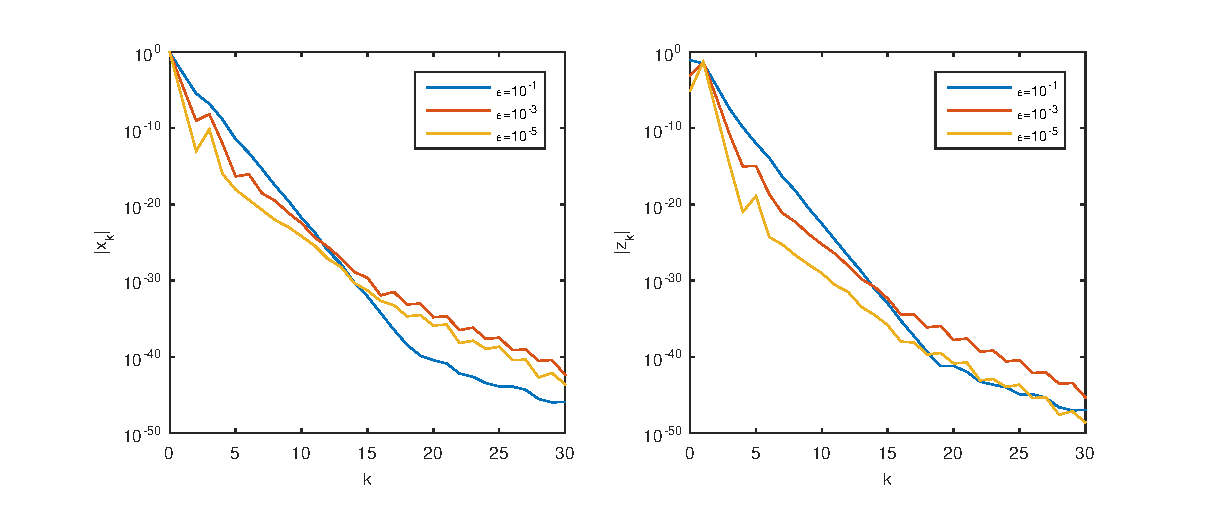
\includegraphics[width=1\textwidth]{img/chap3/norm_coeffs_series.eps}
\caption{Norme infinie des coefficients $(x_k\eeps)$ et $(z_k\eeps)$ en fonction de $k$ dans le cas \eqref{pb:edo_partic_1}.}
\label{fig:norm_coeffs_series}
\end{figure}
On voit alors qu'on peut choisir un rang maximal $k_{\max} = 20$ dans notre cas. Appliquons maintenant un schéma RK4 au polynôme $(u_k\eeps)_{0\leq k\leq 20}$ à $\dt$ fixé et pour diverses valeurs de $\epsilon$ pour étudier si le bon choix de coefficients suffit à diminuer la raideur du problème pour obtenir des schémas uniformément précis par défaut. 
\begin{figure}[!h]
\centering 
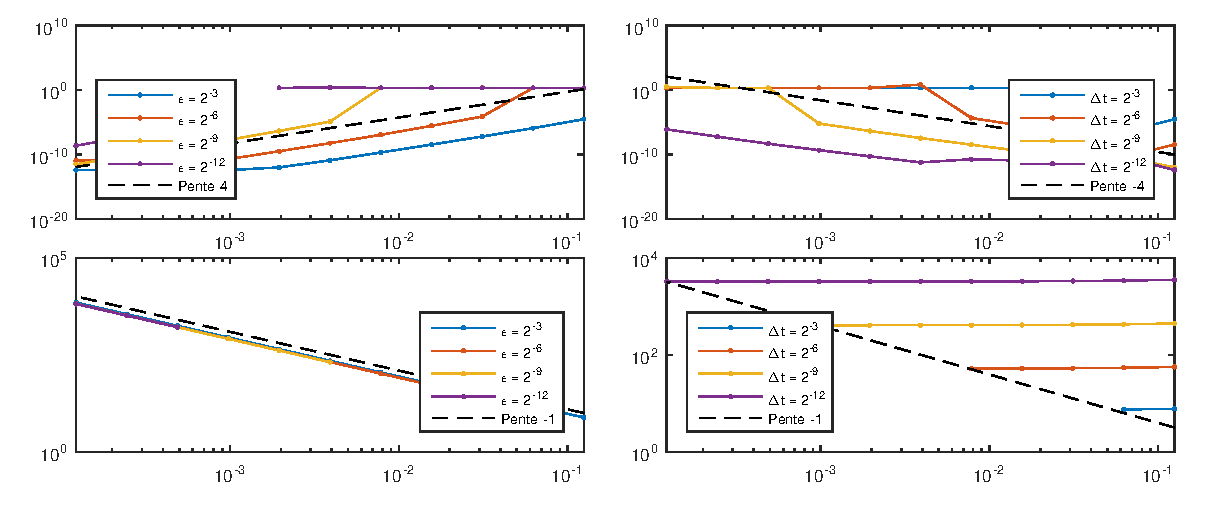
\includegraphics[width=\textwidth]{img/chap3/conv_rk4_series.eps}
\caption{Erreur relative en norme infinie sur $x$ (en haut) et erreur absolue en norme infinie sur $z$ (en bas) en fonction de $\dt$ (à gauche) et de $\epsilon$ (à droite) pour le cas \eqref{pb:edo_partic_1} avec un schéma RK4 sur les $(u_k\eeps)$.}
\label{fig:conv_series_cas1}
\end{figure}
On voit sur la figure \ref{fig:conv_series_cas1} que ce n'est absolument pas le cas, et que la convergence est la même qu'en considérant le système d'origine, sans séries. 
La stabilité est directement liée à $\dt/\epsilon$. 
On observe cela sur l'erreur de $z$ en fonction de $\epsilon$, où tracer une droite $\sim 1/\epsilon$ passe par le dernier point avant que la solution ne diverge pour différentes valeurs de $\dt$. 


\subsection{Implémentation par différences finies}

On voit qu'on peut restreindre l'ensemble de définition de $\tau$ à $[0,\Tk/\epsilon]$. Il faut donc discrétiser ce segment. 
Afin de profiter de la forme exponentielle des fonctions, on choisit une discrétisation de la forme 
$$ \tau_n = -C\ln(\xi_n) $$ 
avec $(\xi_n)_{0\leq n \leq N_{\tau}}$ une dicrétisation uniforme de $[e^{-\Tk/\epsilon},1]$ (décroissante pour avoir $(\tau_n)$ croissante), et $C$ une constante positive qui permet d'avoir une meilleure résolution sur les fonctions de base $(\tau\mapsto e^{-k\tau}), k\in\N$ et $(\tau\mapsto e^{-j\mu\tau}),j\in\N^*$. 
On choisit $C = \max(1/\mu,1)$ pour un bon compromis après une rapide étude de l'erreur d'intégration (avec la formule du trapèze) sur ces fonctions. \\

\subsubsection{Intégration du schéma}

On voit que la seule partie un peu difficile à implémenter pour le schéma sont les produit de convolution par $\tau\mapsto e^{-\mu\tau}$ et $\tau\mapsto e^{-(\mu+1)\tau}$. 
On approxime 

$$ \begin{array}{rl} \displaystyle
\int_0^{\tau_n} e^{-\mu(\tau_n-\sigma)}h(\sigma)d\sigma =& \displaystyle \sum_{k=0}^{n-1} \int_{\tau_{k}}^{\tau_{k+1}} e^{-\mu(\tau_n-\sigma)}h(\sigma)d\sigma \\
\simeq & \displaystyle \sum_{k=0}^{n-1} \left(\int_{\tau_k}^{\tau_{k+1}} e^{\mu(\sigma-\tau_n)} d\sigma \right)\frac{h(\tau_k)+h(\tau_{k+1})}{2}
\end{array} $$
soit pour le schéma, 
$$ Q_{\mu}[0]^{-1}h(\tau) \simeq \sum_{k=0}^{n-1} e^{-\mu\tau_n}(e^{\mu\tau_{k+1}}-e^{\mu\tau_k}) \frac{h(\tau_k)+h(\tau_{k+1})}{2}, $$
$$ S_{\mu}[0]^{-1}h(\tau) \simeq \frac{\mu}{\mu+1}\sum_{k=0}^{n-1} e^{-(\mu+1)\tau_n}(e^{(\mu+1)\tau_{k+1}}-e^{(\mu+1)\tau_k}) \frac{h(\tau_k)+h(\tau_{k+1})}{2}. $$

\begin{remark}
Si on voulait effectuer ce produit de convolution entre deux fonctions discrétisées, l'implémentation serait compliquée puisque la discrétisation n'est pas uniforme. 
En effet, dans le cas d'une discrétisation régulière on aurait 
$ \int_0^{\tau_n} a(\tau-\sigma)b(\sigma)d\sigma = \sum_{k = 0}^{n-1} \frac{\Delta\tau}{2} (a(\tau_n-\tau_k)b(\tau_k) + a(\tau_n - \tau_{k+1})b(\tau_{k+1})) + \O(\tau_n \Delta\tau^2)$ par règle du trapèze. 
Dans le cas d'une discrétisation non uniforme, on n'a pas forcément accès aux valeurs en $\tau_n-\tau_k$, ce qui rend cela impossible. 
\end{remark}

Une fois ces calculs faits, on implémente le schéma et on peut évaluer l'erreur. 

\subsubsection{Étude de l'erreur} \label{sec:err_loc_df}
On veut s'assurer que le schéma permet effectivement de résoudre le système \eqref{pb:EDO_var_cent} avec une précision uniforme. 
Pour cela, on calcule l'erreur pour diverses valeurs de $\dt$ et de $\epsilon$ sur le cas particulier \eqref{pb:edo_partic_1}, avec $N_{\tau} = 2^{10}$ (sachant que dans \cite{chartier2015UA}, la discrétisation est à $32 = 2^5$ points et les résultats sont bons). 

\begin{figure}[!h]
\centering\hspace*{-1.3cm}
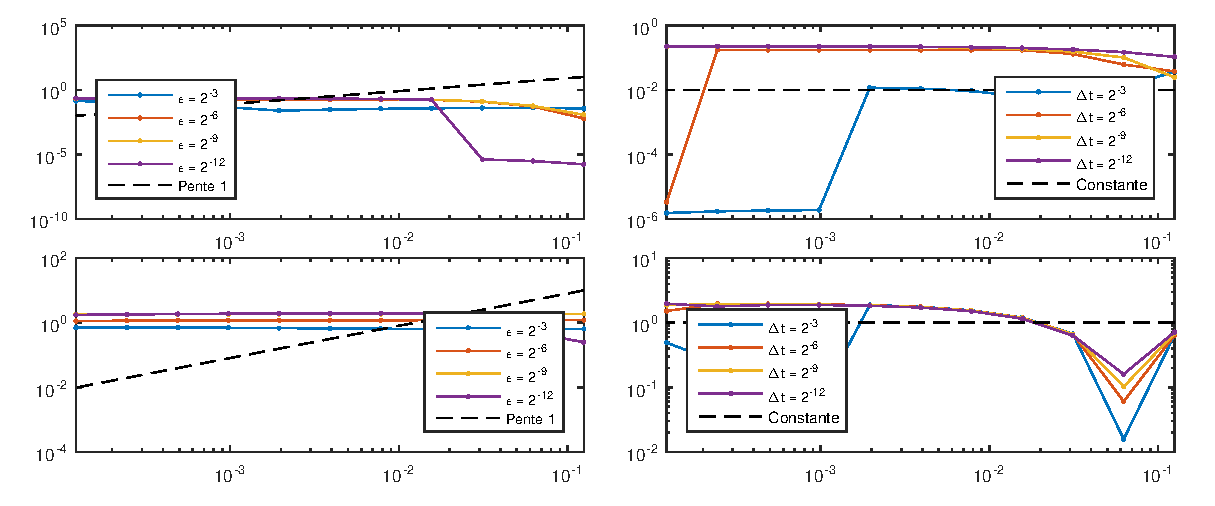
\includegraphics[width=\textwidth]{img/chap3/conv_rel_df_cas1.eps}
\caption{Erreur relative en norme absolue sur $x$ (en haut) et sur $z$ (en bas) en fonction de $\dt$ (à gauche) et de $\epsilon$ (à droite) pour le cas \eqref{pb:edo_partic_1} avec un schéma par différences finies.}
\label{fig:conv_interp_cas1}
\end{figure}

On voit sur la figure \ref{fig:conv_interp_cas1} que le nombre de points $N_{\tau}$ est insuffisant pour espérer avoir une quelconque convergence, malgré le fait qu'il soit élevé. 
On se rend compte que diminuer $\dt$ et $\epsilon$ nécessite d'augmenter $N_{\tau}$, ce qui rend l'utilisation de cette implémentation presque impossible : 
on peut avoir $\dt$ et $\epsilon$ arbitrairement faibles donc il n'est pas possible techniquement d'augmenter $N_{\tau}$ en accord ---et c'est absurde étant donné qu'on souhaite avoir une complexité indépendante de~$\epsilon$. 


\section{Implémentation avec la librairie \texttt{chebfun}}

Puisque l'approche par discrétisation n'a pas fonctionné, on décide d'utiliser la bibliothèque \texttt{chebfun}\cite{chebfun} sur \bsc{Matlab}. 
Cette bibliothèque utilise des interpolations par morceaux avec des polynômes de Chebychev pour effectuer des opérations quasi-exactes sur les fonctions. 
Son utilisation est simple et elle est très utile pour ce qu'on veut faire, mais on ne contrôle pas la complexité des opérations qui peut devenir très élevée dans le cas de fonctions raides. 

Cette fois-ci le calcul du produit de convolution se fait simplement avec la commande \texttt{conv}, ce qui rend l'implémentation aisée. 


\subsection{Erreur globale sur l'équation à variété centrale}

De même qu'avec les différences finies, on calcule l'erreur pour diverses valeurs de $\dt$ et de $\epsilon$ sur le cas particulier \eqref{pb:edo_partic_1}. 
\begin{figure}[!h]
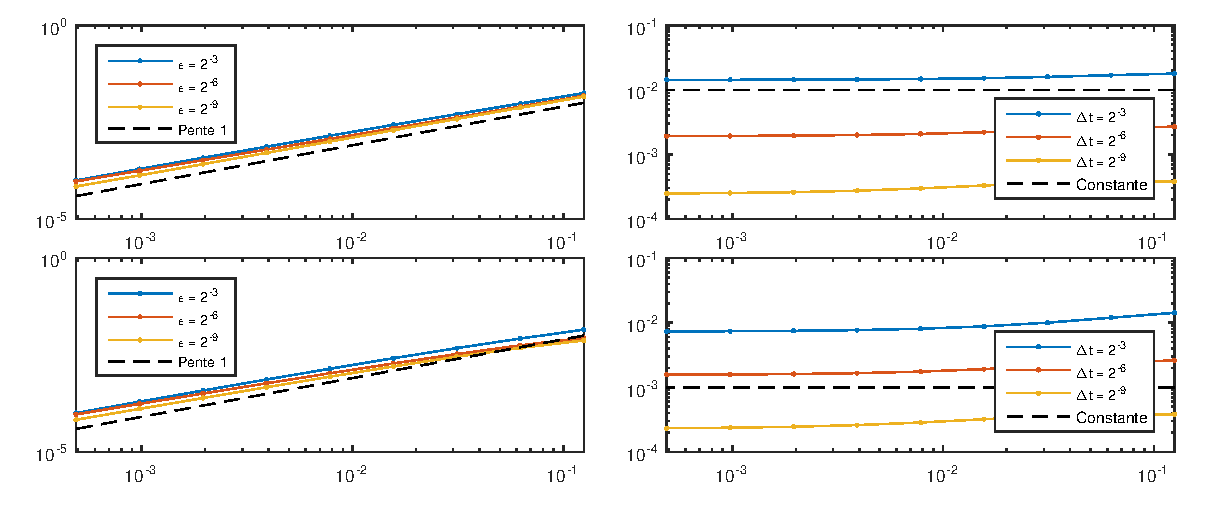
\includegraphics[width=\textwidth]{img/chap3/cheb/conv_rel_cheb_cas1.eps}
\caption{Erreur relative en norme infinie sur $x\eeps$ (en haut) et sur $z\eeps$ (en bas) en fonction de $\dt$ (à gauche) et de $\epsilon$ (à droite) pour le cas \eqref{pb:edo_partic_1} avec le schéma utilisant \texttt{chebfun}.}
\label{fig:conv_cheb_cas1}
\end{figure}

On voit que les résultats obtenus (en figure \ref{fig:conv_cheb_cas1}) sont ceux escomptés, à l'exception d'une légère perte d'ordre. 
On observe bien une convergence d'ordre 1 avec une erreur indépendante de $\epsilon$ comme assuré par le théorème \ref{thm:err_glob}. 
Observons le comportement sur un autre exemple, en choisissant $n=2,m=1$,

\begin{equation} \label{pb:edo_partic_2}
\left\{ \begin{array}{l}
f(x,z) = (1-z)\begin{pmatrix} 0 & -1 \\ 1 & 0 \end{pmatrix} x , \\
g(x,z) = x_1^2 x_2^2 \vphantom{\displaystyle\sum^0}
\end{array} \right. 
\qquad \text{et} \qquad 
\left\{ \begin{array}{l}
x_0 = \begin{pmatrix} 0,1 \\ 0,7 \end{pmatrix} , \\
z_0 = 0,05 . \vphantom{\displaystyle\sum^0}
\end{array} \right.
\end{equation}
%
On trace les mêmes courbes d'erreur en figure \ref{fig:conv_cheb_cas1}. 
\begin{figure}[!h]
\centering
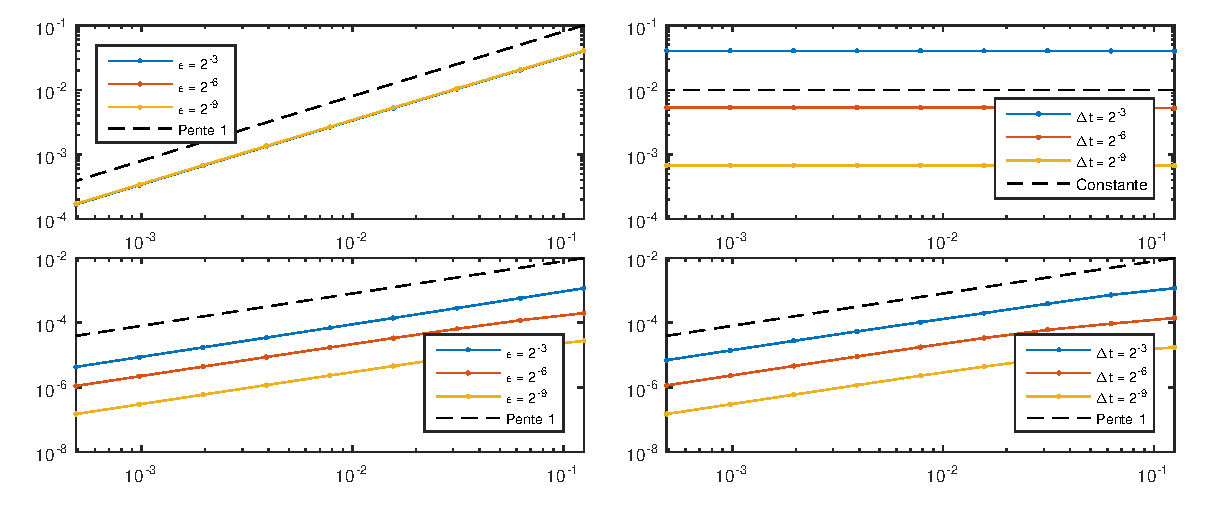
\includegraphics[width=\textwidth]{img/chap3/cheb/conv_abs_cheb_cas2.eps}
\caption{Erreur absolue en norme infinie sur $x$ (en haut) et sur $z$ (en bas) en fonction de $\dt$ (à gauche) et de $\epsilon$ (à droite) pour le cas \eqref{pb:edo_partic_2} avec le schéma utilisant \texttt{chebfun}.}
\label{fig:conv_cheb_cas2}
\end{figure}
Le schéma est uniformément précis d'ordre 1 pour le problème à variété centrale avec cette implémentation. 
On trace l'erreur absolue car la fonction $z\eeps$ s'annule en certains points et donc l'erreur relative est mal calculée, comme on le voit sur la figure \ref{fig:erreur_cheb_cas2}. 
\begin{figure}[!h]
\centering
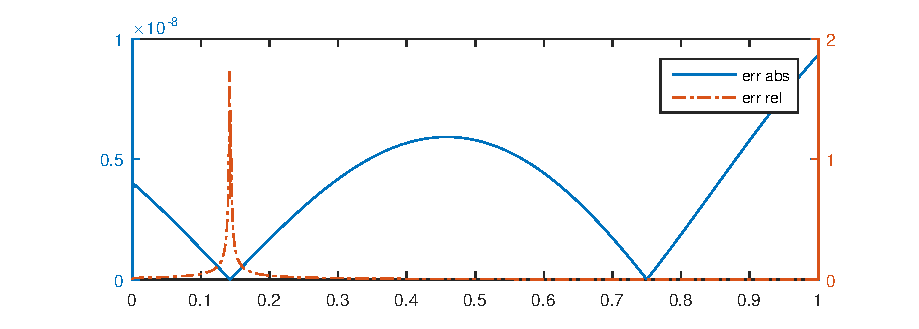
\includegraphics[scale=.85]{img/chap3/cheb/errors_cheb_cas2.eps}
\caption{Erreurs absolue (trait plein) et relative (pointillés) et leur échelle respectives à gauche et à droite en fonction du temps après calcul avec l'implémentation \texttt{chebfun} avec $\dt = 2^{-10}$ et $\epsilon = 2^{-14}$.}
\label{fig:erreur_cheb_cas2}
\end{figure}
Dans cet exemple, l'erreur relative, localisée sur un zéro, est d'ordre $1$ alors que l'erreur absolue est d'ordre $10^{-8}$. 
On voit néanmoins sur la figure \ref{fig:conv_cheb_cas2} que l'erreur absolue sur $z\eeps$ évolue en $\O(\epsilon\dt)$, ce qui est cohérent avec le fait que $z\eeps$ converge vers une fonction d'ordre $\epsilon$ en temps long. \\

Observons l'efficacité de cette approche utilisant \texttt{chebfun} sur les fonctions de $\tau$ directement, pour vérifier la robustesse de notre implémentation. 


\subsection{Erreur locale sur l'équation de transport}

On suppose que dans le premier cas test, les solutions obtenues avec \texttt{chebfun} sont exactes et on cherche à vérifier l'erreur locale en $\O(\dt^2)$.

On calcule de façon symbolique les fonctions $\tilde{X}\eeps(\dt,\cdot), \tilde{Z}\eeps(\dt,\cdot)$ obtenues après un seul pas de temps et on les compare à $X\eeps(\dt,\cdot),Z\eeps(\dt,\cdot)$ calculées avec notre schéma en utilisant un pas de temps $\dt_{qe} \ll \dt$. 
Si $X\eeps(\dt,\cdot),Z\eeps(\dt,\cdot)$ sont effectivement quasi-exactes, alors l'erreur sera d'ordre $\O(\dt^2)$. 

Pour le calcul symbolique, on passe par la transformée de Laplace puis la transformée inverse. 
On pourrait effectuer une intégration directe, mais cela permet d'introduire rapidement une nouvelle approche, qu'on pourra développer pour une autre implémentation après ce stage. 
En effet, puisque $\mathcal{L}\{\dptau h\}(\xi) = \xi \mathcal{L}\{h\}(\xi) - h(0)$, on a 
$$ \mathcal{L}\{X_1\eeps\}(\xi) + \frac{1}{\mu} \left( \xi \mathcal{L}\{X_1\eeps\}(\xi) - X_B(\dt) \right) = \mathcal{L}\{\dt f(X_0\eeps,Z_0\eeps) + X_0\eeps\}(\xi) $$
d'où 
\begin{equation} \label{eq:laplace_X}
\mathcal{L}\{X_1\eeps\}(\xi) = \frac{1}{\xi+\mu}\left( X_B(\dt) + \mu\mathcal{L}\{\dt f(X_0\eeps,Z_0\eeps) + X_0\eeps\}(\xi) \right) 
\end{equation}
et on peut appliquer une transformée de Laplace inverse pour obtenir $X_1\eeps$. De la même manière on a 
\begin{equation} \label{eq:laplace_Z}
\mathcal{L}\{Z_1\eeps\}(\xi) = \frac{1}{\xi+\mu+1}\left( Z_B(\dt) + \mu\mathcal{L}\{\dt g(X_0\eeps,Z_0\eeps) + Z_0\eeps\}(\xi) \right). 
\end{equation}

Avec cette approche, on est absolument certain que la solution numérique après un pas de temps est exacte. 
On effectue l'étude pour quelques valeurs $(\dt_i)$, la solution quasi-exacte étant calculé avec un pas de temps $\dt_{qe} = 2^{-10}\min(\dt_i)$. 

\begin{figure}[!h]
\centering
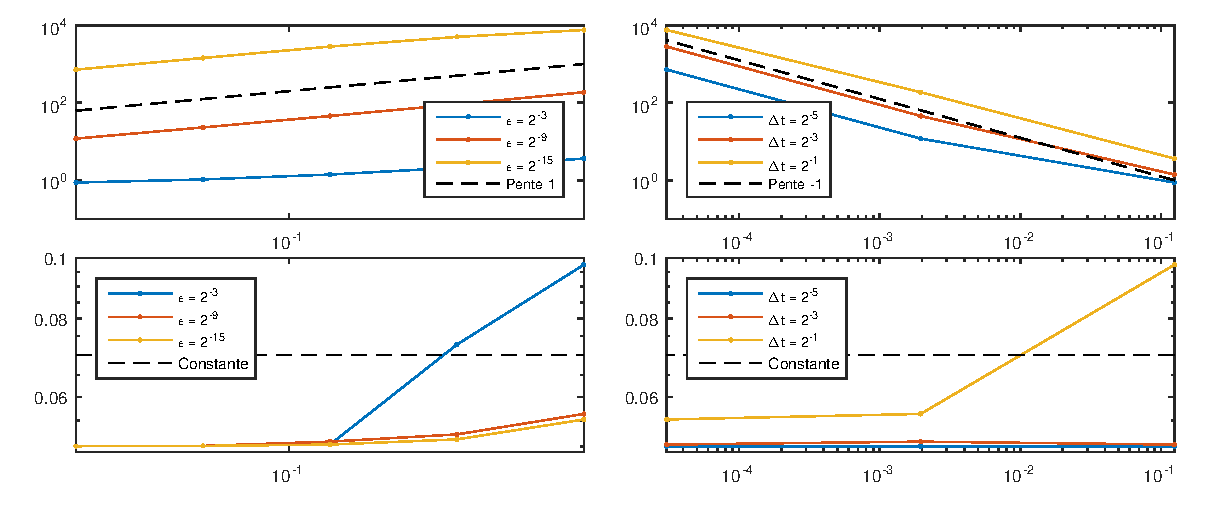
\includegraphics[width=\textwidth]{img/chap3/cheb/conv_cheb_one_step_cas1.eps}
\caption{Différence en norme $\Linftau$ entre la solution <<~quasi-exacte~>> calculée avec \texttt{chebfun} et la solution calculée symboliquement avec un seul pas de temps pour $X\eeps(\dt,\cdot)$ (en haut) et $Z\eeps(\dt,\cdot)$ (en bas) en fonction de $\dt$ (à gauche) et de $\epsilon$ (à droite).}
\end{figure}

On voit que le résultat n'est pas du tout celui auquel on s'attendait: on n'observe pas vraiment de convergence, l'erreur est toujours très grande, avec un plateau pour $\epsilon$ grand et $\dt$ petit. 
En outre, même pour $\dt,\epsilon$ grands, au lieu d'avoir une convergence en $\O(\dt^2)$ on observe une dépendance en $\O(\dt/\epsilon)$. 

Malheureusement, les temps de calcul sont très long et donc on ne peut pas effectuer les calculs avec $\dt_{qe}$ plus faible. 
Une observation plus précise des fonctions de $\tau$ calculées nous montre qu'elles deviennent de plus en plus raides en $\tau = 0$ au fil des itérations. 
On ne sait pas si cela est dû à l'implémentation ou au schéma directement. 
En effet, on n'a pas de relation pour évaluer $\|\dptau U_n\eeps\|$ en fonction de $n$, donc le schéma pourrait causer des fonctions difficiles à représenter numériquement, ce qui pourrait accentuer ce type d'erreurs. 

Cette interprétation n'explique cependant pas pourquoi l'erreur dépend de $\epsilon$. 
Probablement que le problème est accentué lorsque $\mu$ est petit. 

Étant donné que le schéma converge quand même pour la solution du système d'origine \eqref{pb:EDO_var_cent}, on peut se pencher sur les coûts et les conséquences liées à son implémentation dans un cadre <<~réel~>>.


\subsection{Coût de l'implémentation}

Notre implémentation n'est pas forcément très pratique, puisque la librairie \texttt{chebfun} est puissante mais coûteuse (en termes d'opérations), et elle n'est disponible que pour \textsc{Matlab}. 
On souhaite néanmoins en évaluer le coût opérationnel en fonction de $\dt,\epsilon$. Notre méthode est la suivante: 

\begin{itemize} 
\item On applique le schéma avec $\dt$ et $\epsilon$ fixés et on mesure le temps pris par les calculs. 
\item On mesure les erreurs absolue et relative sur $u = (x,z)$ grâce à une solution quasi-exacte calculée avec le schéma Radau IIA. 
\item On calcule une solution avec le schéma Radau en utilisant des tolérances absolue et relative de l'ordre des erreurs obtenues par le schéma et on mesure le temps de calcul. 
\end{itemize} 
Les calculs sont effectués sur un processeur Intel Core i5-6500U @ 2.30 GHz, à 2 c\oe{}urs. 
À notre connaissance, un seul processus était utilisé, même pour les opérations de \texttt{chebfun}. 
Cette procédure est répétée pour différentes valeurs de $\dt,\epsilon$ pour obtenir des courbes similaires à celles d'erreur en figure \ref{fig:cost_cheb_cas1}. 
\begin{figure}[!h]
\centering 
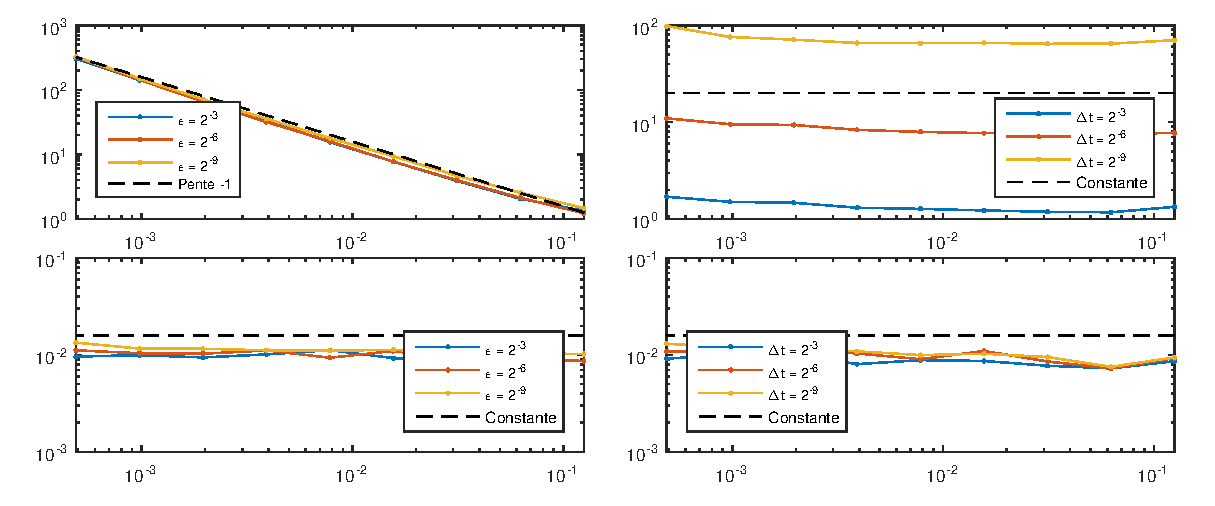
\includegraphics[width=\textwidth]{img/chap3/cheb/cost_cheb_cas1.eps}
\caption{Temps de calcul en secondes de la solution avec \texttt{chebfun} (en haut) et avec Radau IIA (en bas) en fonction de $\dt$ (à gauche) et de $\epsilon$ (à droite).}
\label{fig:cost_cheb_cas1}
\end{figure}

La première remarque qu'on peut faire est que le temps de calcul de la solution avec Radau IIA est toujours au moins 2 ordres de grandeur en dessous de celui pris pour notre schéma. 
On voit aussi que le temps de calcul avec Radau est presque indépendant de la tolérance (proportionnellement liée à $\dt$) et de $\epsilon$. 
On voit que le temps de calcul augmente un peu à mesure que $\epsilon$ diminue pour le schéma Radau et pour l'implémentation avec \texttt{chebfun}, mais de façon très faible. 

\section{Pistes de recherche}

Ce stage se poursuivant en thèse, il nous reste quelques idées à étudier plus profondément qu'on n'a pas encore pu développer. 

\subsection{Discrétisation du domaine de Laplace}

On a vu rapidement qu'on pouvait utiliser la transformée de Laplace pour résoudre le schéma numérique. Il y a quelques soucis liés à cette approche:
\begin{enumerate}
\item Le domaine de Laplace est de dimension 2, ce qui rend sa discrétisation plus coûteuse qu'en 1D,
\item La bibliographie autour de la transformée de Laplace numérique et son inverse est assez peu référencée, 
\item Les schémas impliquant cette transformée sont très rares, ce qui peut rendre l'approche difficile à accepter par la communauté, 
\item On a besoin d'un calcul direct et inverse rapide, avec une discrétisation de $[0,\Tk/\epsilon]$ adaptée pour pouvoir calculer $f(X_n,Z_n)$ et $g(X_n,Z_n)$ à chaque itération. Cela amène des questions : 
\begin{itemize}
\item Comment définir <<~adaptée~>>? 
\item Comment trouver une telle discrétisation de façon dynamique? 
\end{itemize} 
On a vu qu'une discrétisation fixe n'était pas adaptée au problème avec l'approche par différences finies.
\end{enumerate}
On voit ainsi que cette direction apporte de nombreuses problématiques à creuser, ce qui la rend à la fois attractive et difficile à aborder. 

L'argument principal en faveur de cette approche est que la transformée de Laplace peut être vue comme l'équivalent de la transformée de Fourier du cas périodique dont on s'inspire. 
En effet, la transformée de Laplace permettrait d'extraire facilement les coefficients d'une série $\sum_{k\geq 0} u_k e^{-k\tau}$ pour $\tau\in\R_+$ de la même manière que la transformée de Fourier avec les séries $\sum_{k\geq 0} u_k e^{-ik\theta}$ pour $\theta\in\R/P\mathbb{Z}$. 
Or on a vu qu'on pouvait essentiellement se ramener à des séries exponentielles pour résoudre le système \eqref{pb:EDO_var_cent}, ce qui permettrait peut-être de fabriquer des méthodes <<~spectrales~>> (il en existe pour le cas hautement oscillant). 


\subsection{Schéma local à coût plus faible}

Face à ce problème, on essaie d'appliquer un autre schéma, qui ne calcule pas $X\eeps,Z\eeps$ directement, mais qui peut peut-être servir pour $x\eeps,z\eeps$. 
L'idée est simple, même si l'étude théorique n'a pas été effectuée : il s'agit d'appliquer seulement la première étape du schéma, en boucle. Ainsi on pose 
$X_n\eeps(\tau) = x_n\eeps + \epsilon\int_0^{\tau} [f(x_n\eeps,e^{-\sigma}z_n\eeps) - f(x_n\eeps,0)]d\sigma$ et $Z_n\eeps(\tau) = e^{-\tau}z_n\eeps + \epsilon\int_0^{\tau} e^{\sigma-\tau} [g(x_n\eeps,e^{-\sigma}z_n\eeps) - \dpz g(x_n\eeps,0)\cdot e^{-\sigma}z_n\eeps]d\sigma$ et on peut calculer 
$$ x_{n+1}\eeps = e^{-\mu\dt/\epsilon} b_{\dt}^{(x)}(x_n\eeps,z_n\eeps) + \mu\int_0^{\dt/\epsilon} e^{-\mu(\dt/\epsilon - \sigma)} \big(\dt\, f(X_n\eeps(\sigma),Z_n\eeps(\sigma))+X_n\eeps(\sigma)\big) d\sigma $$
$$ z_{n+1}\eeps = e^{-(\mu+1)\dt/\epsilon} b_{\dt}^{(z)}(x_n\eeps,z_n\eeps) + \mu\int_0^{\dt/\epsilon} e^{-(\mu+1)(\dt/\epsilon-\sigma)} \big(\dt g(X_n\eeps(\sigma),Z_n\eeps(\sigma))+Z_n\eeps(\sigma)\big) d\sigma $$
où $b_{\dt}^{(x)}(x_n\eeps,z_n\eeps)$ et $b_{\dt}^{(z)}(x_n\eeps,z_n\eeps)$ donnent la valeur des conditions au bord calculées comme dans \eqref{eq:CB_XZ} en remplaçant $x_0,z_0$ par $x_n\eeps,z_n\eeps$, ces conditions au bord étant évaluées en $\dt$. 

En cas de convergence, cette approche permet une implémentation algébrique simple, au coût indépendant de $\epsilon$. 
En effet, ces nouvelles fonctions $X_n\eeps,Z_n\eeps,f(X_n\eeps,Z_n\eeps),g(X_n\eeps,Z_n\eeps)$ sont naturellement des séries exponentielles d'après leur définition, donc le seul cas particulier à considérer pour l'approche algébrique est $\mu\in\N$, ce qui n'est pas un frein. 

Le problème opérationnel de ce schéma est qu'il implique deux intégrations par pas de temps: une pour calculer $X_n\eeps,Z_n\eeps$ et une pour $x_{n+1}\eeps,z_{n+1}\eeps$. 
Ces intégrations étant simples, il semble plutôt efficace quand même. 
Cependant on aurait souhaité limiter le nombre d'intégrations étant donné que les schémas dans le cas hautement oscillant n'en effectuant qu'une par pas de temps. 

Néanmoins, ce schéma se présente comme assez simple à étudier théoriquement et à implémenter tout en pouvant fournir des résultats convaincants.
On a en effet pu l'implémenter très facilement en utilisant \texttt{chebfun} et on a observé une précision uniforme sur nos deux cas particuliers. 
Cela en fait une piste de recherche prioritaire. 

